\section{Results}
Our first hypothesis predicted that when human and robot work were interdependent, human workers would have a more positive attitude toward robots and the resulting collaboration than when their work were independent. Our analyses provided support for this hypothesis; we found that when human and robot work depended on each other, participants rated the robot as being significantly more competent, $F(1,20) = 6.54$, $p = .0187$, and expressed marginally more willingness to collaborate with the robot, $F(1, 20) = 3.74$, $p = .0676$, compared to when there was no interdependency. We found no differences across different levels of task interdependence in other measures.

Our second hypothesis was that participant attitudes toward robotic teammates and the resulting collaboration would be more positive when collaborating on specialized, non-homogeneous tasks than in collaborations on non-specialized, homogeneous tasks. Consistent with our hypothesis, we found that when participants and the robot worked on non-homogeneous tasks, they rated the robot to be significantly more competent compared to when they worked on homogeneous tasks, $F(1,20) = 4.86$, $p = .0393$. Data from other measures provided did not vary across different levels of task homogeneity.

\begin{figure}[!th]
	\caption{Data from measures of perceived competence, willingness to collaborate, and perceived task load that highlight the main findings of our analyses. $^\dagger$ and $^*$ denote significant and marginal differences, respectively.}
	\label{fig:data}
	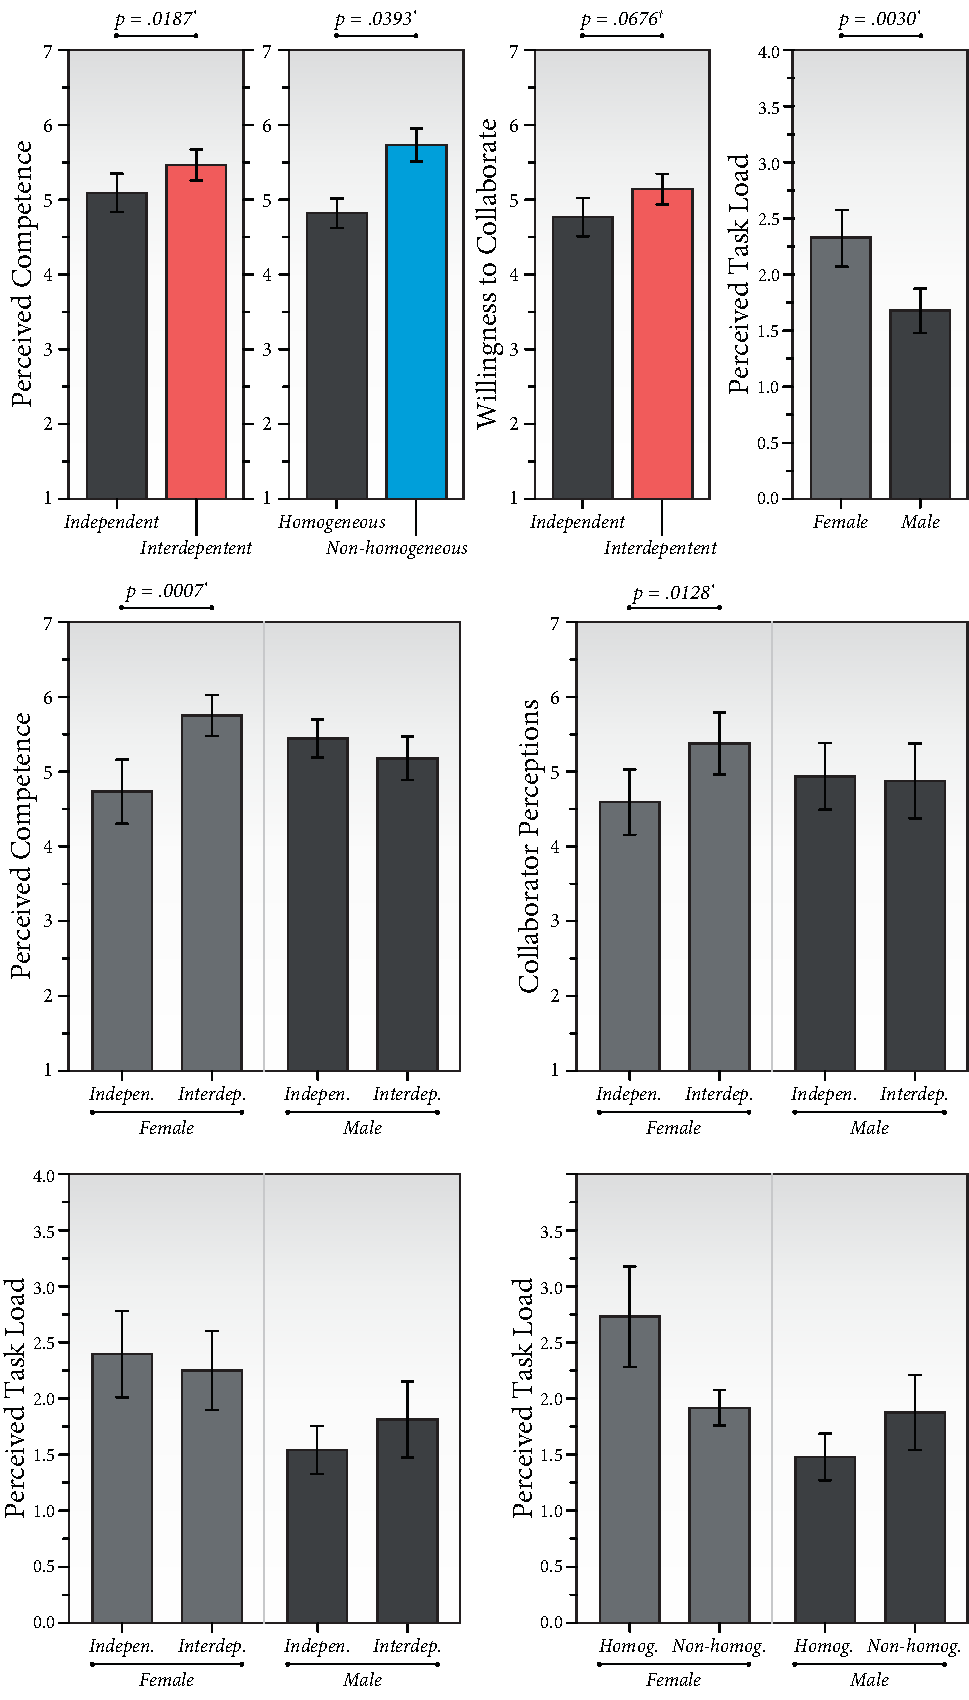
\includegraphics[width=\columnwidth]{figures/hri18-aksari-figures_data-figures.pdf}
\end{figure} 

As noted in the Hypothesis Section, we also conducted an exploratory analysis of the effects of worker sex on worker experience, as prior work in human-robot collaboration point toward significant differences in the attitudes of men and women toward robots \cite{mutlu2006task,mutlu2006storytelling,schermerhorn2008robot,takayama2009influences}, which we expected to observe in the manufacturing setting. This exploratory analysis revealed that task characteristics had a differential effect on how men and women perceived of the robot and the task. Specifically, we found an interaction effect between participant sex and task dependency over perceptions of the robot's competence, $F(1,20)=10.50$, $p=.0041$, and a marginal interaction between over participants' willingness to collaborate with the robot, $F(1,20)=4.18$, $p=.0543$. Comparisons across levels of task interdependence for each gender showed that female participants were significantly more willing to collaborate with the robot when their work depended on the robot's work than when it did not, $F(1,20) = 7.4694$, $p = .0128$, $\alpha_{ajd}=0.025$.
%$F(1,28) = 4.18$, $p = 0.054$
They also found the robot to be significantly more competent when their work depended on that of the robot, $F(1,20) = 15.91$, $p = .0007$, $\alpha_{ajd}=0.025$.
%$F(1,28) = 5.16$, $p = 0.032$
Data from male participants did not differ across different levels of task dependency.
Our exploratory analysis also found a main effect of sex on perceived task load, women reporting their task load to be significantly higher than men, $F(1,20) = 11.41$, $p = 0.0030$. We also found an interaction effect between participant sex and task homogeneity over perceptions of the task load, $F(1,20) = 6.98$, $p = 0.0156$, although comparisons for each gender did not find significant differences in perceived task load across different levels of task homogeneity.

Finally, we also report on the effects of demographic factors on measured psychological outcomes of human-robot teaming in order to identify other individual differences future research might investigate. Our analyses showed that the frequency with which participants played computer games significantly predicted perceived competence of robot, $F(1,20) = 7.83$, $p = 0.011$, willingness to collaborate with the robot, $F(1,20) = 10.39$, $p = 0.004$, and perceived contribution of the robot, $F(1,20) = 7.25$, $p = 0.014$, while negatively significantly predicting task load, $F(1,20) = 7.69$, $p = 0.0117$. Participant comfort with assembly tasks significantly predicted perceived competence of the robot, $F(1,20) = 7.54$, $p = 0.0124$, and familiarity with robots significantly predicted willingness to collaborate with the robot, $F(1,20) = 5.27$, $p = 0.033$.

